\section{Experimental Apparatus}\label{sec:experiment}
The DUET experiment used the M11 beam line at TRIUMF which produced a $\pi^{+}$ beam of $>$99\% purity at five different momentum settings between 201.6 MeV/c and 295.5 MeV/c. An extensive description of the beamline, beam particle identification, and the PIA$\nu$O detector can be found in Sec. II of \cite{duet}. Fig.  \ref{fig:config} shows a schematic overview of the experimental apparatus.
%Particle identification was obtained by combining time-of-flight (TOF) information and relative light yield in a Cherenkov detector placed in the beam path. 

\begin{figure}[ht]
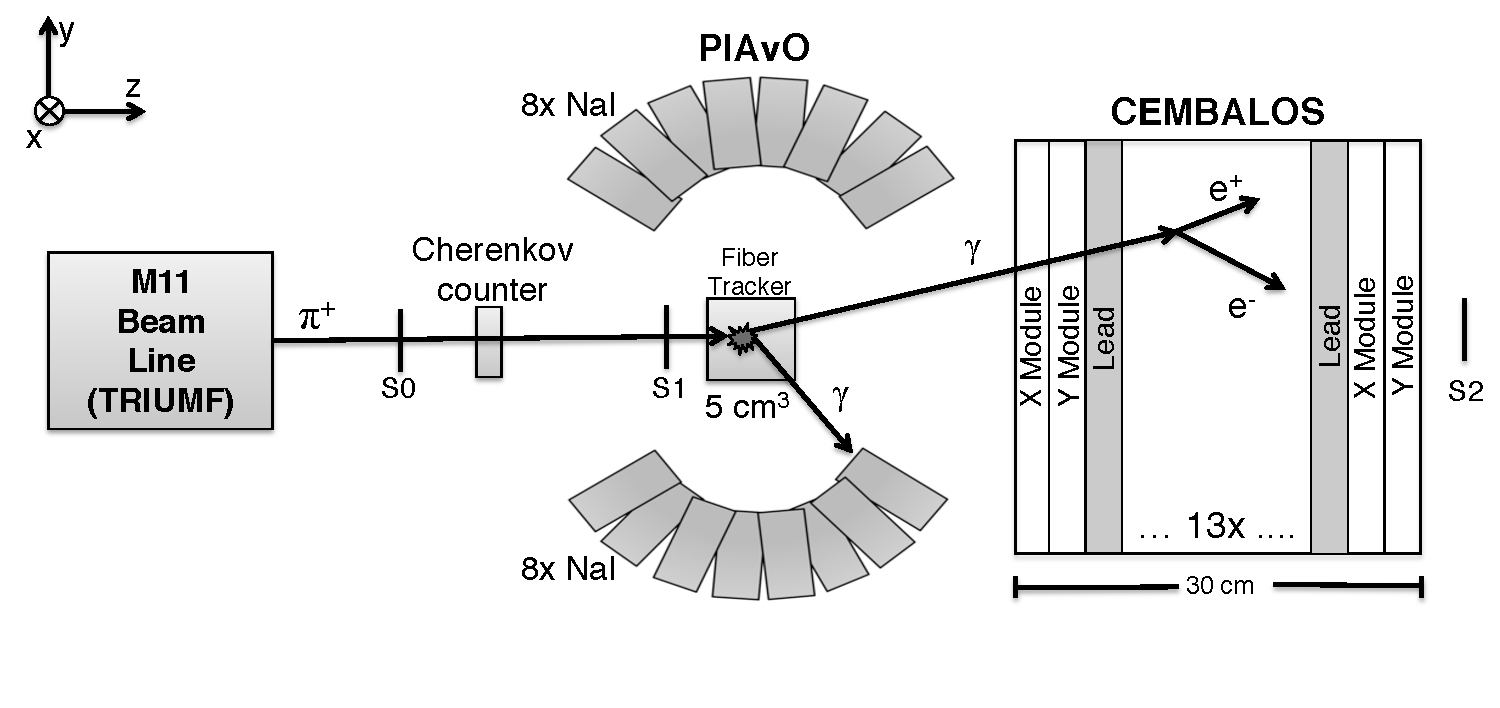
\includegraphics[width=90mm]{figures/duet_schematic_forpaper_v2.pdf}
\caption{Schematic overview of the experimental apparatus.}
\label{fig:config}
\end{figure}

%\begin{figure}[!h]
%\begin{center}
%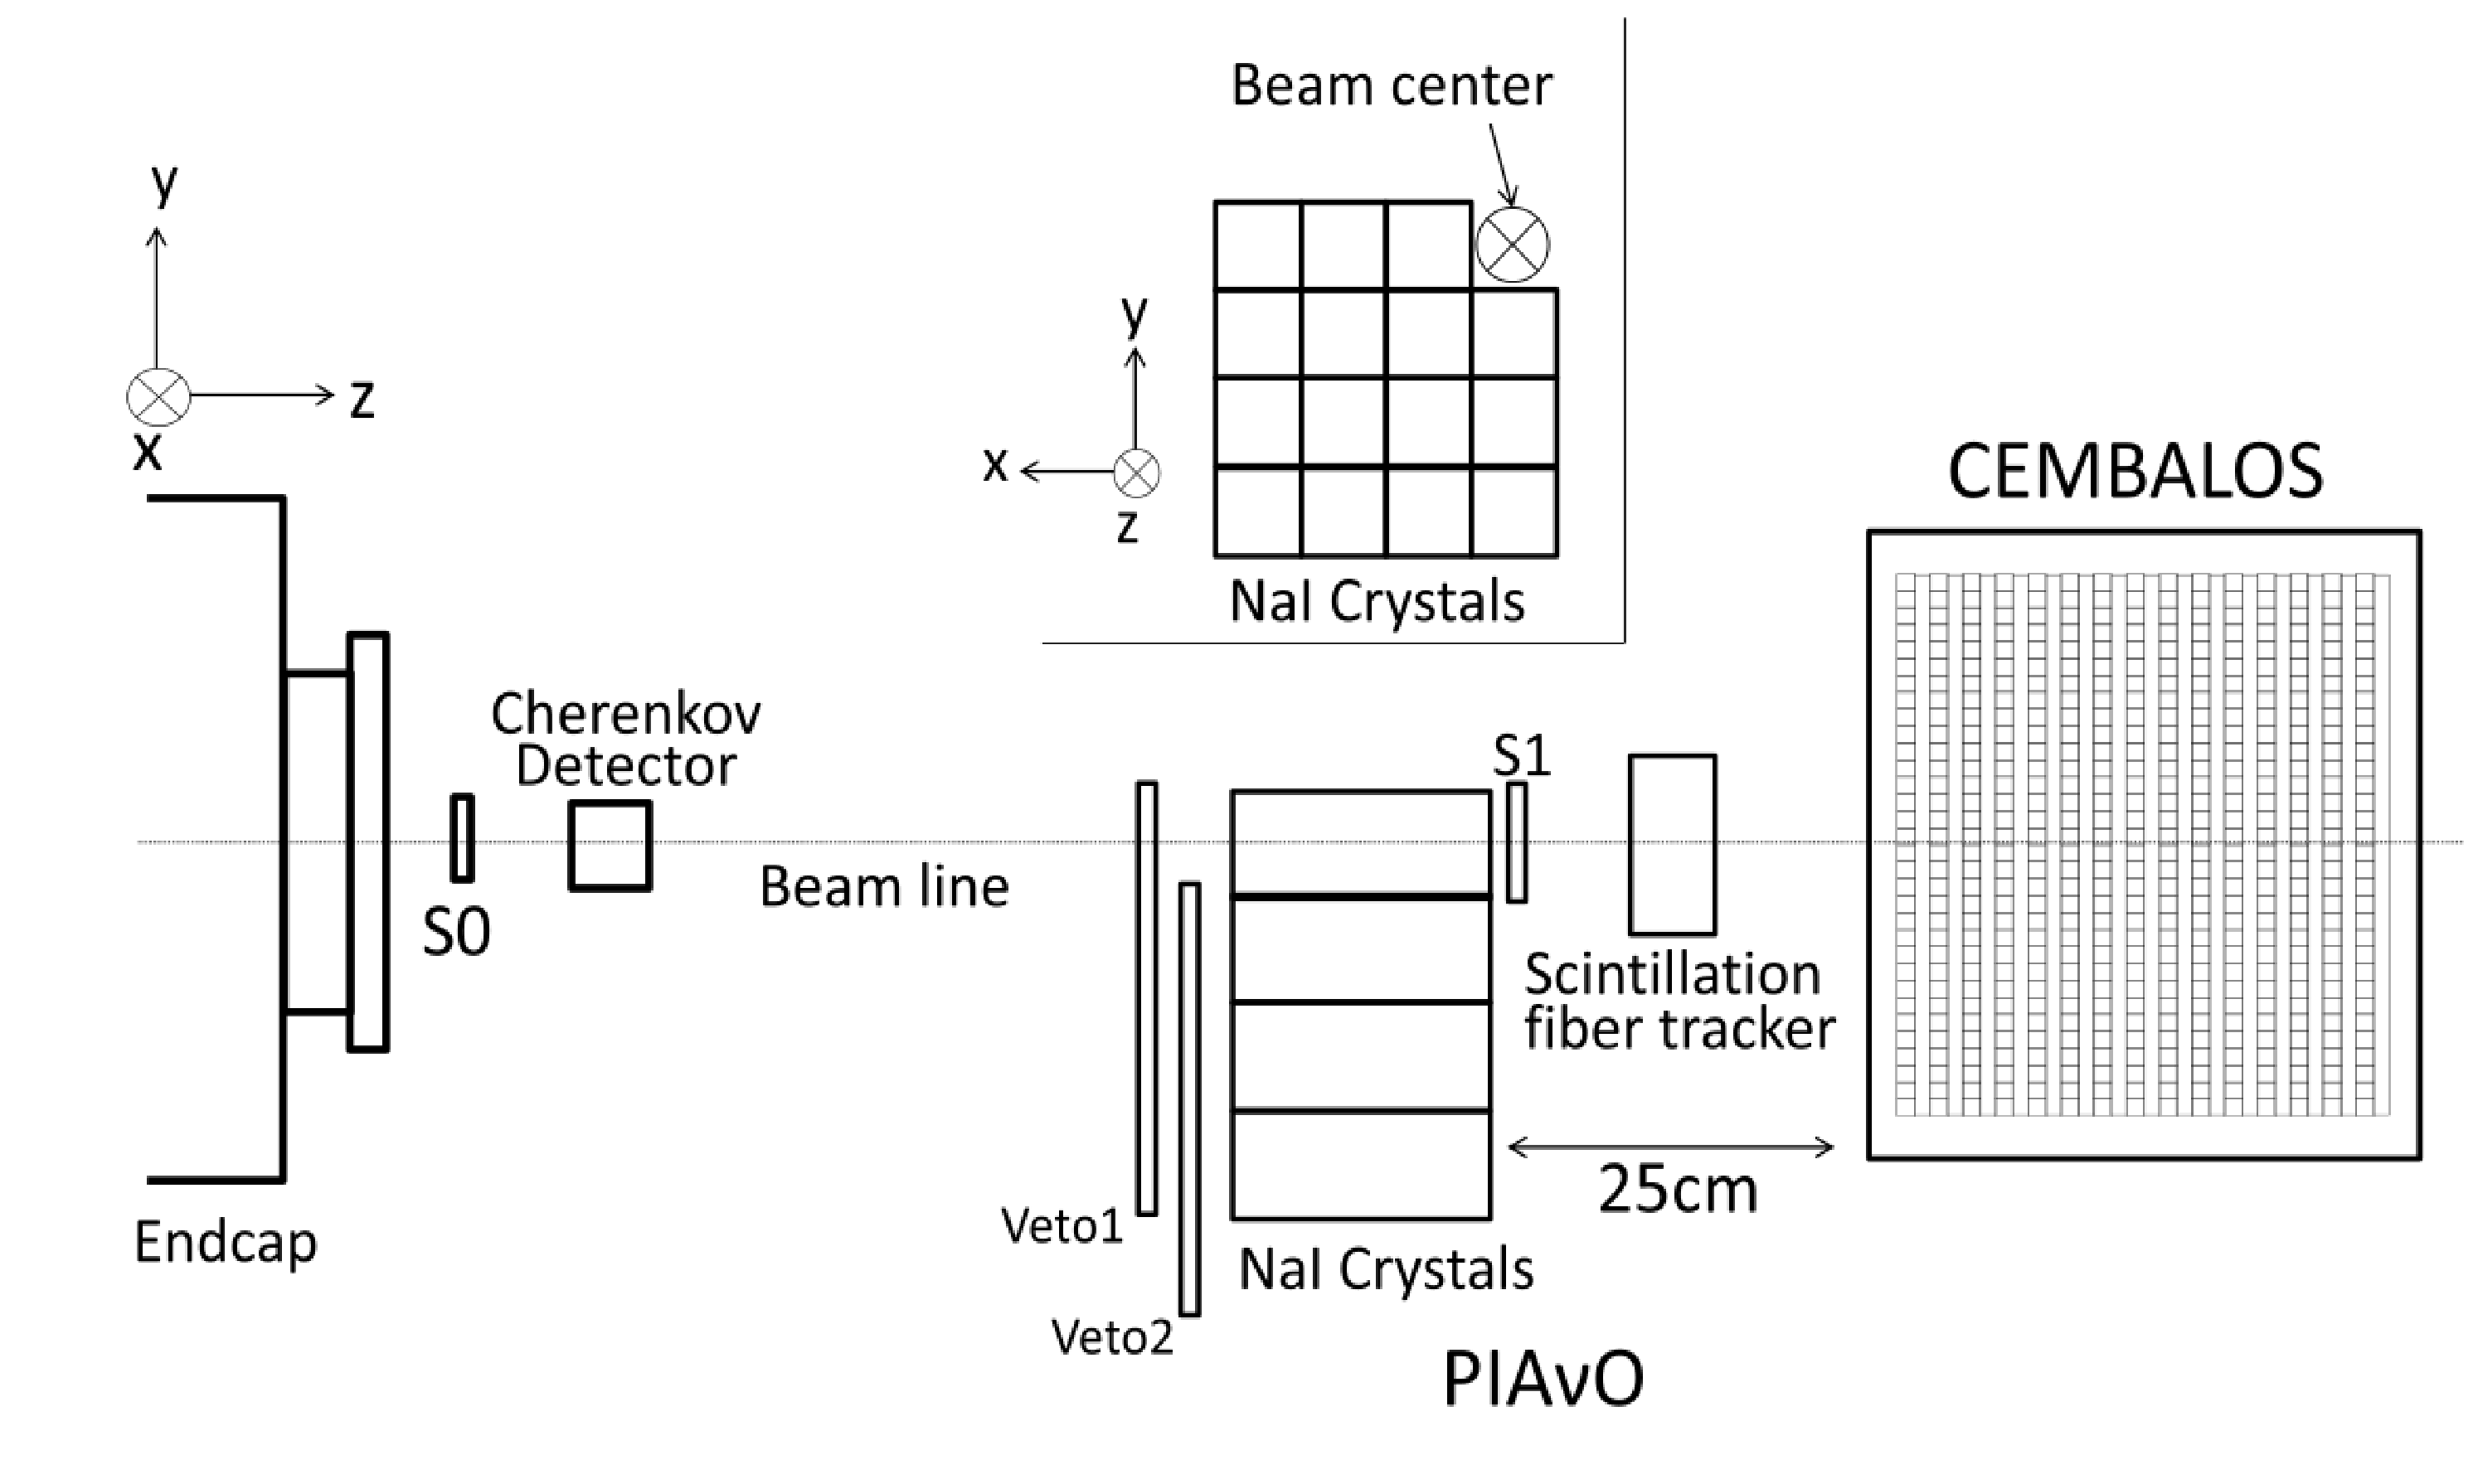
\includegraphics[width=80mm]{figures/duet_setup3.eps}
%\caption{Apparatus layout. Detailed description in the text.\label{fig:config}}
%\end{center} 
%\end{figure}

PIA$\nu$O (PIon detector for Analysis of neutrino Oscillation) served as an active carbon target for pion interactions and  provided excellent tracking capabilities and $dE/dx$ measurements of charged particles. It provided sufficient information to select ABS+CX events by requiring no observed $\pi^{+}$ in the final state. It consisted of 16 horizontal and 16 vertical layers of scintillating material, each with 32 fibers. The dimension of the region where the fibers cross each other was $\sim5\times5\times5$ cm$^3$, providing $(1.518\pm0.007)\times10^{24}$ carbon target nuclei in its fiducial volume. The scintillation light from the fibers was read out by multi-anode photomultiplier tubes. 16 NaI crystal detectors were placed around the tracker region but are not used for this analysis.

The forward-going photons following the decay of a $\pi^0$ produced in a CX interaction were identified using the CEMBALOS (Charge Exchange Measurement By A Lead On Scintillator) detector.

\subsection{CEMBALOS}
The CEMBALOS detector was a scaled down (1/6) version of the Fine-Grained Detectors (FGDs) \cite{fgd} of T2K. It was located 25cm downstream of PIA$\nu$O. Its core component were scintillator bars made of polystyrene co-extruded with a 0.25 mm thick reflective coating of polystyrene doped with TiO$_2$. The light yield from the far end of a bar was measured to be up to 16-18 photoelectrons (p.e.) for a minimum ionizing particle. The optical crosstalk through the TiO$_2$ coating between bars was measured to be 0.5$\pm$0.02\%. 

The scintillator bars were arranged into 15 XY modules oriented perpendicular to the beam. Each XY module contained 32 bars in the $x$ direction glued to 32 bars in the $y$ direction. Layers of 0.25mm thick fiberglass (G10) were glued to both the upstream and downstream surfaces to provide support, and no adhesive was applied between the bars. Each module had dimensions of 32$\times$32$\times$2.02 cm$^3$. Unlike the FGDs, 0.8$\sim$1 mm thick lead layers were interspersed in between each module to enhance photon conversion. 
%Figure \ref{fig:cembalos} shows a picture of CEMBALOS.

%\begin{figure}[!h]
%\begin{center}
%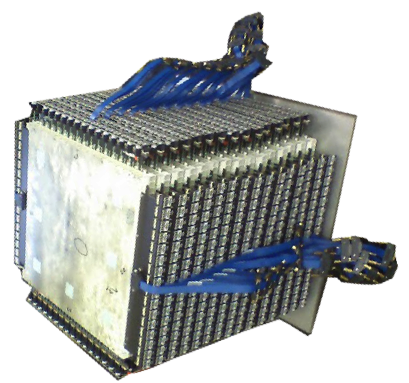
\includegraphics[width=80mm]{figures/cembalos_photo.png}
%\caption{(Color online) Photograph of CEMBALOS. The beam points to the right. Detailed description in the text.\label{fig:cembalos}}
%\end{center} 
%\end{figure}

The scintillation light from each bar was collected by a 1 mm$\pm$2\% diameter wavelength (WLS) double-clad Kuraray Y11 (200) S-35 J-type fiber inserted through an axial hole. The absorption and subsequent emission wavelengths for these fibers were 430 nm and 476 nm, respectively. Unlike the FGDs, due to limited availability only fibers in the last 3 XY modules had one of their ends mirrored to enhance light collection by aluminizing.

Multi-Pixel Photon Counters (MPPCs) manufactured by Hamamatsu Photonics (S10362-13-050C) were used as photosensors to measure the scintillation light. These provided excellent photon counting capability with higher quantum efficiency than photo-multipliers for the spectra of light produced by the WLS fibers. Its outer dimensions were 5mm$\times$6mm, while the sensitive area was 1.3mm$\times$1.3 mm$^2$ containing 667 avalanche photo-diode pixels. The small size allowed for using one MPPC per bar, eliminating the possibility of crosstalk at the sensor. A custom connector was developed to achieve good optical coupling.
The XY modules were hung inside an aluminum light-tight box. The read out electronics were mounted on the outer sides of the box to separate elements generating heat and to prevent temperature induced effects to the MPPCs. 
%(Add information about the support structure)

%The MPPCs were mounted on busboards. Each busboard contained 16 MPPCs, 2 temperature sensors and 16 LEDs for calibration. The MPPCs were read out by X "Mini-crates" connected using ribbon cables. Each mini-crate contained: 1) Front-end board (FEB) to set the bias voltage for the MPPCs (64 channels/board) and to digitize and store the waveforms using an AFTER ASIC chip that provided a preamplifier, a shaper and a switched capacitor array for each channel; 2) crate master board (CMB) to control the data acquisition process using a Xilinx Virtex 2 Pro FPGA chip; 3) a light pulser board to control LEDs on the busboard used for gain calibration of the MPPCs. Each CMB was connected to a data concentrator card (DCC) based on a Xilinx-IV FPGA with a PPC405/300Mhz microprocessor and a Gigabit Ethernet port. A MIDAS \cite{midas} front-end program ran directly on the DCCs and handled the transfer of data to a back-end computer for permanent storage. 

\subsubsection{\bf Detector simulation and calibration}\label{section:calibration}
The simulation of the CEMBALOS detector was based on that developed for the FGDs used by T2K. It made use of the \textsc{Geant4} version 9.4 patch 04~\cite{geant} simulation toolkit. Details of the geometry of the detector were simulated, including, but not limited to, the fiber structure (core, double cladding and coating), the G10 layers and the glue used to hold them to the fibers and the measured thickness of the interspersed lead layers.

The energy deposit from charged particles traversing the scintillating fibers was calculated from the pulse height ($PH$) of the digitized MPPC waveforms by the following procedure:

\begin{enumerate}
\item {\it Conversion from PH to photoelectrons:} The $PH$ measured in ADC units were translated into the number of photoelectrons $N_{pe}$ by normalizing to the average pulse height $\left\langle PH \right\rangle$ corresponding to a single-pixel avalanche. 
\begin{equation}
N_{pe} = PH/\left\langle PH \right\rangle
\end{equation}
The distribution of dark noise pulse heights was used to measure $\left\langle PH \right\rangle$ and it was found to be 48.65 ADC units. 
\item{\it Corrections for variations in overvoltage:} Temperature variations can change the overvoltage, the difference between the operating and breakdown voltages in the MPPCs, affecting the photon detection efficiency and the crosstalk and after-pulsing probabilities. Empirical corrections were applied to compensate for these effects.
\item{\it Correction for saturation of the MPPCs:} Since each MPPC has a finite number of pixels, the pulse height can get saturated. A correction based on an exponential decaying empirical expression was applied.
\item{\it Correction for bar-to-bar variations:} Minor variations in the fiber-MPPC coupling, scintillation material, fiber mirroring, diameter of the hole, etc. can introduce a difference in the light yield for each bar. Those variations are accounted by an additional correction representing the factor by which the efficiency for conversion of energy deposition in the bar to number of photons hitting the MPPCs differs from its value averaged over all the bars in CEMBALOS.
\item{\it Correction for light loss along the bar: } The light attenuation in each fiber was measured for both mirrored and unmirrored bars using cosmic rays. Fig. \ref{fig:attcurves} shows the resulting fitted distributions for the measured yield ($N_{DPE}$) of detectable photoelectrons as a function of the distance of the hit to the MPPC. The fit function is an empirical descriptor of the attenuation process.
\begin{figure}[!h]
\begin{center}
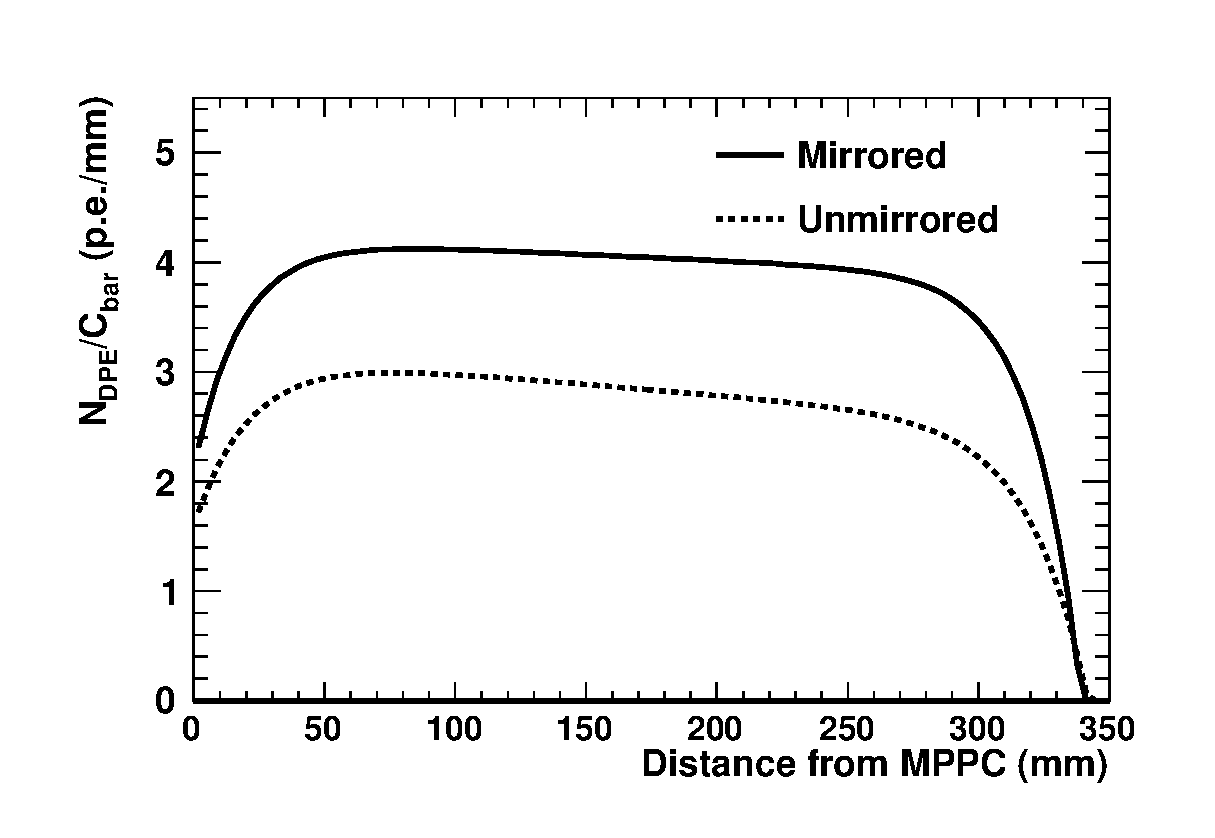
\includegraphics[width=85mm]{figures/attcurves_paper.eps}
\caption{Light attenuation curves in CEMBALOS for mirrored (solid) and unmirrored (dashed) fibers}
\label{fig:attcurves}
\end{center} 
\end{figure}
\end{enumerate}

The calibration steps described corrected MPPC responses which are assumed to be proportional to the number of scintillation photons. The final conversion to energy deposition measured in p.e. involved  an empirical normalization constant and Birk's formula was used to account for the nonlinearity in the scintillator response. We adopted 0.0208$\pm$0.0003(stat)$\pm$0.0023(sys) cm/MeV for the value of Birk's constant as measured by the SciBar Collaboration \cite{scibar}. A minimum of 5 p.e. was required to label an energy deposit as a hit.

A control sample of beam muons in the $p_{\pi}$=237.2 MeV$/c$ setting traversing CEMBALOS was used to calibrate the charge simulation. Fig. \ref{fig:muoncharge} shows the deposited charge distribution of through-going muons for data and MC after the calibration procedure. The agreement is satisfactory.
%At least 4 hits on both the first and last 5 layers were required. The angular distributions of the reconstructed tracks in CEMBALOS for data and MC agree.

\begin{figure}[!h]
\begin{center}
%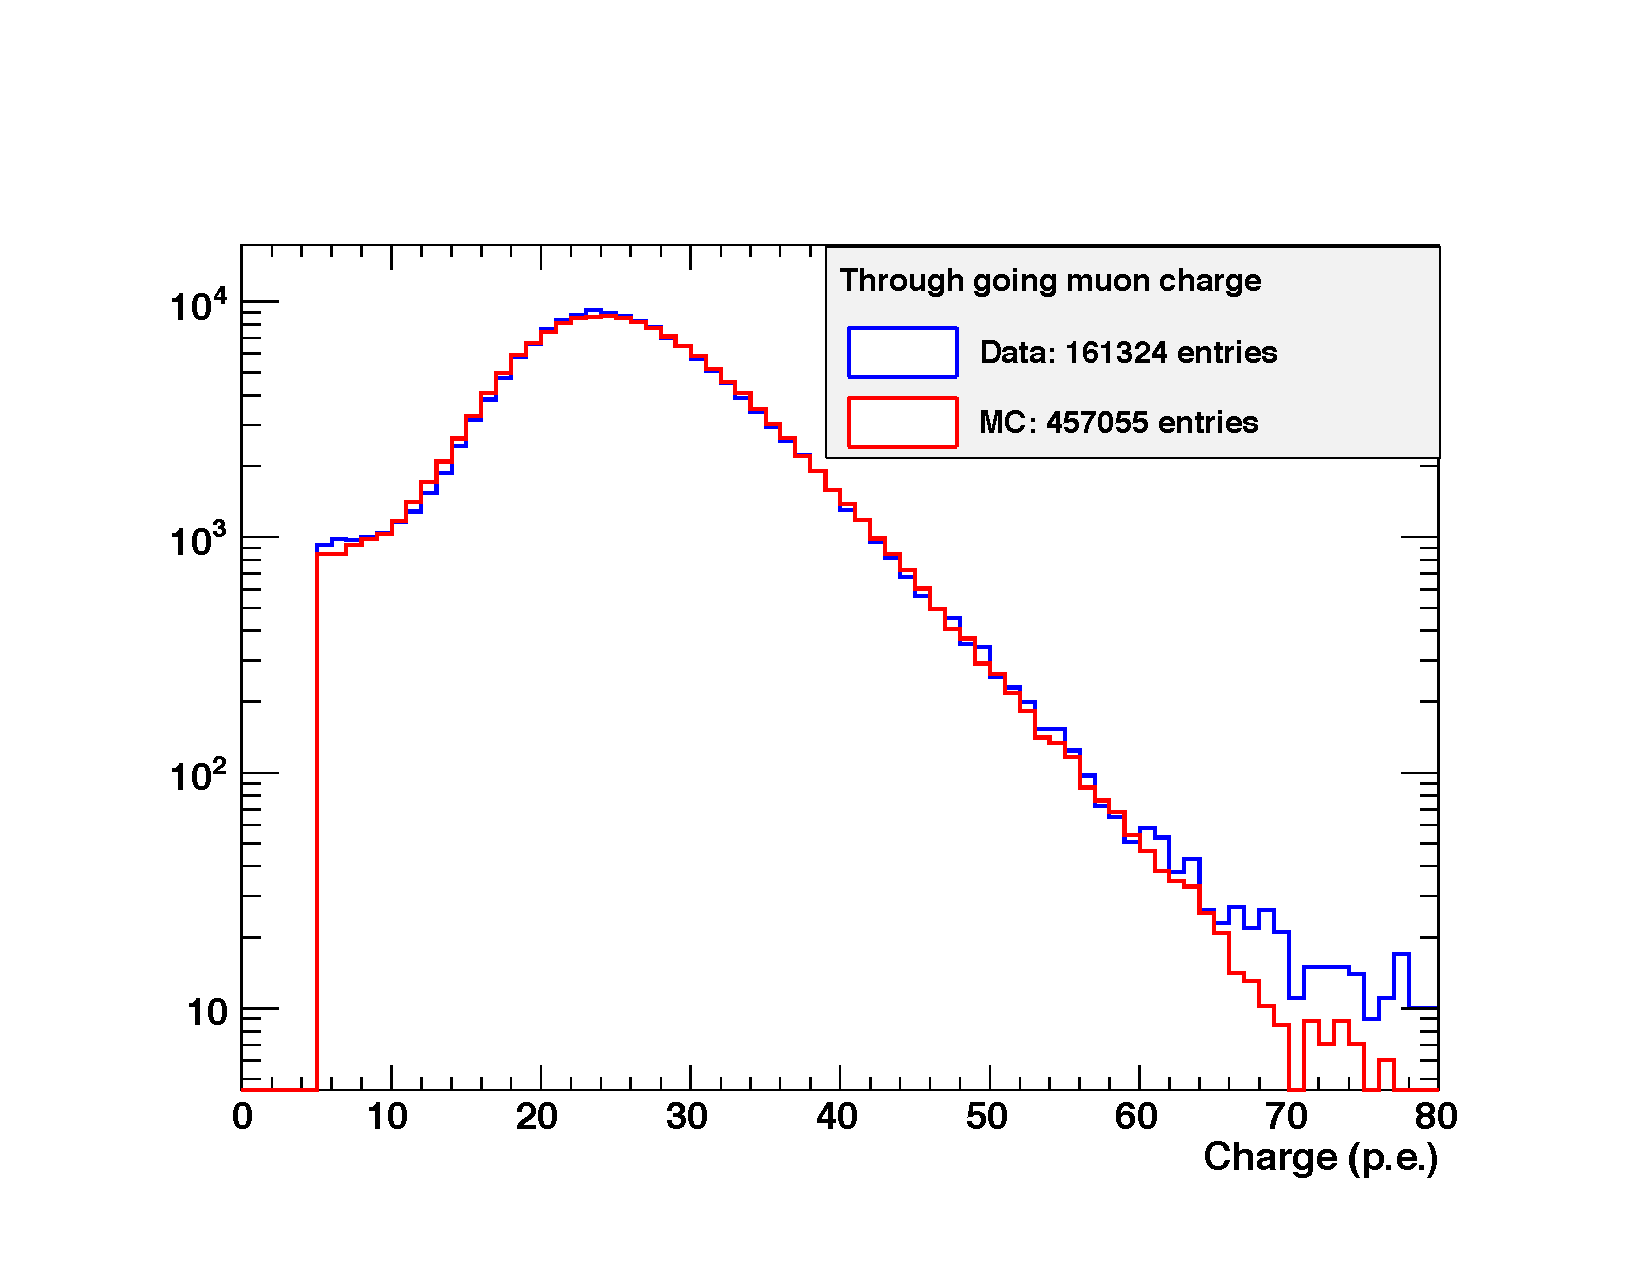
\includegraphics[width=80mm]{figures/muoncharge.pdf}
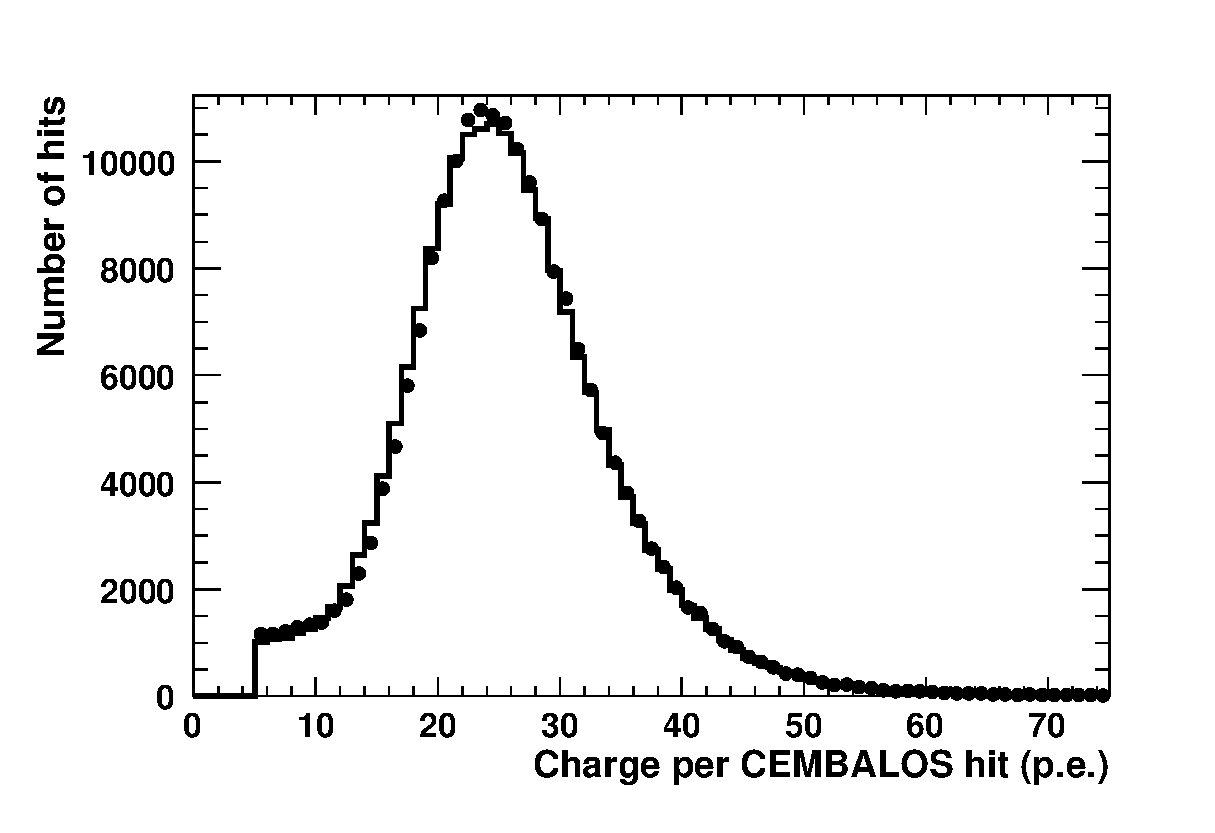
\includegraphics[width=85mm]{figures/muon_charge_calib.eps}
\caption{CEMBALOS deposited charge distribution (in photoelectrons) of through-going muons in the $p_{\pi}$=237.2 MeV$/c$ setting for data (circles) and MC (solid line), after the calibration procedure was applied.}
\label{fig:muoncharge}
\end{center}
\end{figure}

\subsection{Event Summary}
The data set used in this analysis is the same as in \cite{duet}. Data was recorded for a $\pi^{+}$ beam on a scintillation (carbon) target for five incident momenta (201.6, 216.6, 237.2, 265.5, 295.1 MeV$/c$). There were $\sim$1.5 million beam triggered events recorded for each momentum setting, except for the 216.6 MeV$/c$ setting where only 30\% was recorded due to limited beam time.
